\documentclass[a4paper]{article}

\usepackage{array}
\usepackage{ctexcap}
\usepackage{ctex}
\usepackage{geometry}
\usepackage{graphicx}
\usepackage{amsmath,amssymb,lastpage,ulem,booktabs}
\usepackage{array,tabularx}
\usepackage{siunitx}
\usepackage{floatrow,calc}
\newcolumntype{C}{>{\hfil}X<{\hfil}}
\geometry{
    top=25mm, 
    left=25mm, 
    right=25mm, 
    bottom=25mm,
    headsep=10mm,
    footnotesep=7mm
}
\title{{\bfseries 电路理论基础实验} \\ \zihao{4}\songti 仪器入门及电位、电压的测量}
\author{材料科学与工程学院\\ 杨越\quad 22301071}
\date{}
\pagestyle{plain}

\begin{document}
\begin{center}
    {\mbox{}\\[7em]\zihao{2}\bfseries\songti%
    电路基础实验实验报告}\\[34mm]
    {\zihao{-3}\bfseries\songti
    实验名称:\uline{\hfill\mbox{元件伏安特性的测试}\hfill} \\[2.9mm]
    学\quad 号:\uline{\makebox[25mm]{22301071}}\hfill
    姓\quad 名:\uline{\makebox[25mm]{杨\quad 越}}\hfill
    班\quad 级:\uline{\makebox[25mm]{22级高分子}} \\[2.9mm]
    合作者:\uline{\makebox[25mm]{杨雨燃}}\hspace*{7.4mm}
    桌\quad 号:\uline{\makebox[25mm]{32}}\hfill\mbox{}\\[2.9mm]
    指导教师:\uline{\makebox[30mm]{张志鹏}}\hfill\mbox{} \\[2.9mm]
    实验日期:\uline{\makebox[30mm]{2024-05-07}}\hfill\mbox{} \\[58.7mm]

    }
\end{center}
\newpage

\section{实验目的}
\begin{enumerate}
    \item 学习线性电阻元件和非线性电阻元件伏安特性的测试方法;
    \item 学习直流稳压电源、万用表、直流电流表、电压表的使用方法。
\end{enumerate}

\section{实验原理及电路图}
\begin{flushleft}
    \bfseries\zihao{-4}\songti 【实验原理】
\end{flushleft}
\begin{enumerate}
    \item 元件的伏安特性:电流-电压关系。\par 取电压为横坐标,电流为纵坐标得到电压电流的关系曲线。
    \item 线性电阻元件:伏安特性曲线表现为通过坐标原点的直线,双向性(与电压电流方向无关),关系上服从欧姆定律。
    \item 非线性电阻元件:伏安特性曲线结果不符合欧姆定律,元件电阻随电压或电流的变化而改变。\par 部分非线性电阻元件的伏安特性与电压或电流方向有关,如二极管等单向元件。\par 常见非线性电阻元件伏安特性分类如下:
        \begin{enumerate}
            \item 电流控制型电阻元件:元件端电压为元件电流的单值函数
            \item 电压控制型电阻元件:元件电流为元件端电压的单值函数
            \item 既是电流控制型又是电压控制型元件:伏安特性曲线是单调增加或减小的
        \end{enumerate}
    \item 伏安特性测量方法,用电流表、电压表测定,称为伏安法。\par 通过改变其中一个变量测量另一变量,其选取与元件类型有关:
        \begin{enumerate}
            \item 电压控制型,改变电压测电流
            \item 电流控制型,改变电流测电压
        \end{enumerate}
    \item 伏安法测量包括:电压表外接法与电压表内接法两种。\par 实际上电表并非理想电表,电压表会产生一定的分流,电流表会占有一定的分压,其测量结果和真实情况可能有所区别,两种方法得到的结果不同,可以通过本实验加以比较。
\end{enumerate}
\begin{flushleft}
    \bfseries\zihao{-4}\songti 【电路图】
\end{flushleft}
\begin{center}
    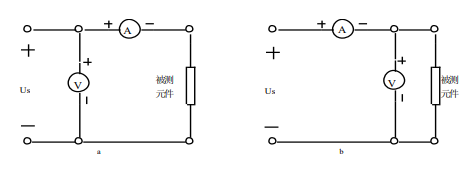
\includegraphics[width=\textwidth-40mm]{001}\\
    \bfseries\zihao{5}\songti 图1:实验电路图(左:电压表外接法,右:电压表内接法)
\end{center}
\newpage

\section{实验仪表}
本实验采用电路原理实验箱《元件伏安特性的研究》单元\par 线性电阻元件:$120\Omega/2W$,$51\Omega/2W$\par 非线性电阻元件:D3(二极管1N5401),D4(发光二极管高亮$\phi3$)

\section{实验内容及步骤}
\begin{enumerate}
    \item 测量线性电阻元件伏安特性(分别采用法1,法2测试,比较测试结果)。
        \begin{enumerate}
            \item 线性电阻元件正向特性测量:根据电路图连接电路,从0开始调到各电压(电流)值,测出对应的电流(电压)值,并将对应的结果填入附表1-4。
            \item 线性电阻元件反向特性测量:改变加在电阻元件两端电压的方向。重复上述内容,并将对应结果填入附表1-4。
            \item 计算对应的电阻值:根据测量的电压、电流值,利用欧姆定律进行计算得到其电阻值。
        \end{enumerate}
    \item 测试非线性电阻元件D3(二极管)、D4(发光二极管)的伏安特性。
        \begin{enumerate}
            \item 正向特性测试:用毫安表和万用表直流50V档分别测量电压与电流,其中元件正极接电流表“-”端,直流稳压电源“+”端接电流表“+”端。分别采用法1、法2进行测量。曲线曲率大的位置测量点密集,反之稀疏,记录对应表格。
            \item 反向特性测试:D3或D4负极接直流电源“+”端,正极接“-”端。测电流用万用表微安档或微安表,测电压用±50V电压表或数字万用表,记录对应表格。
            \item 根据所记录的数据,画出对应非线性电路元件的伏安特性曲线。
        \end{enumerate}

\end{enumerate}

\newpage
\section{实验结果}
    \songti\zihao{-4} 各个实验结果表如下所示,签名页附报告后\par
    \begin{table}[!ht]
        \caption{实验一:线性电阻元件正(反)向特性测量(电流表外接法 R=$120\Omega/2W$)}\label{tab:exp4}
        \begin{tabularx}{\textwidth}{c*{6}{C}} \toprule
            给定电压值(V) & 10 & 8 & 6 & 4 & 2 & 0 \\ \midrule
            测量电流值(mA) & 82.497 & 66.503 & 49.733 & 32.805 & 16.014 & 0 \\计算电阻值($\Omega $) & 121.22 & 120.30 & 120.64 & 121.93 & 124.89 & - \\ 绝对误差($\Omega $) & 1.22 & 0.30 & 0.64 & 1.93 & 4.89 & - \\ \midrule 给定电压值(V)& 0  & -10 & -8 & -6 & -4 & -2 \\ \midrule 测量电流值(mA)& 0  & -81.582 & -64.258 & -47.012 & -29.933 & -14.703 \\计算电阻值($\Omega $) & -  & 122.58 & 124.50 & 127.63 & 133.63 & 136.03\\ 绝对误差($\Omega $) & -  & 2.58 & 4.50 & 7.63 & 13.63 & 16.03 \\
            \bottomrule
        \end{tabularx}
    \end{table}
    \begin{table}[!ht]
        \caption{实验一:线性电阻元件正(反)向特性测量(电流表外接法 R=$51\Omega/2W$)}\label{tab:exp4}
        \begin{tabularx}{\textwidth}{c*{6}{C}} \toprule
            给定电压值(V) & 10 & 8 & 6 & 4 & 2 & 0 \\ \midrule
            测量电流值(mA) & 179.644 & 149.366 & 113.822 & 75.765 & 38.014 & 0 \\ 计算电阻值(Ω) & 55.67 & 53.56 & 52.71 & 52.79 & 52.61 & - \\ 绝对误差($\Omega $) & 4.67 & 2.56 & 1.71 & 1.79 & 1.61 & - \\ \midrule 给定电压值(V) & 0 & -2 & -4 & -6 & -8 & -10 \\ \midrule 测量电流值(mA) & 0 & -38.102 & -76.167 & -114.142 & -151.642 & -187.305 \\ 计算电阻值($\Omega $) & - & 52.49 & 52.52 & 52.57 & 52.76 & 53.39 \\ 绝对误差($\Omega $) & - & 1.49 & 1.52 & 1.57 & 1.76 & 2.39 \\
            \bottomrule
        \end{tabularx}
    \end{table}
    \begin{table}[!ht]
        \caption{实验一:线性电阻元件正(反)向特性测量(电流表外接法 R=$120\Omega/2W$)}\label{tab:exp4}
        \begin{tabularx}{\textwidth}{c*{6}{C}} \toprule
            给定电压值(V) & 10 & 8 & 6 & 4 & 2 & 0 \\ \midrule
            测量电流值(mA) & 77.691 & 62.551 & 45.627 & 31.194 & 15.818 & 0 \\ 
            计算电阻值($\Omega $) & 128.72 & 127.90 & 131.50 & 128.23 & 126.44 & - \\   
            绝对误差($\Omega $) & 8.72 & 7.90 & 11.50 & 8.23 & 6.44 & - \\ \midrule 给定电压值(V) & 0 & -2 & -4 & -6 & -8 & -10 \\ \midrule 测量电流值(mA) & 0 & -15.733 & -30.816 & -45.617 & -62.04 & -75.542 \\ 
            计算电阻值($\Omega $) & - & 127.12 & 129.80 & 131.53 & 128.95 & 132.38 \\ 
            绝对误差($\Omega $) & - & 7.12 & 9.80 & 11.53 & 8.95 & 12.38 \\
            \bottomrule
        \end{tabularx}
    \end{table}
    \begin{table}[!ht]
        \caption{实验一:线性电阻元件正(反)向特性测量(电压表外接法 R=$120\Omega/2W$)}\label{tab:exp4}
        \begin{tabularx}{\textwidth}{c*{6}{C}} \toprule
            给定电压值(V) & 10 & 8 & 6 & 4 & 2 & 0 \\ \midrule
            测量电流值(mA) & 167.212 & 128.455 & 92.904 & 55.599 & 19.096 & 0 \\ 
            计算电阻值($\Omega $) & 59.80 & 62.28 & 64.58 & 71.94 & 104.73 & - \\ 
            绝对误差($\Omega $) & 8.80 & 11.28 & 13.58 & 20.94 & 53.73 \\ \midrule
            给定电压值(V) & 0 & -2 & -4 & -6 & -8 & -10 \\ \midrule
            测量电流值(mA) & 0 & -31.024 & -72.69 & -108.451 & -141.541 & -174.292 \\ 
            计算电阻值($\Omega $) & - & 64.47 & 55.09 & 55.32 & 56.52 & 57.37 \\ 
            绝对误差($\Omega $) & - & 13.47 & 4.09 & 4.32 & 5.52 & 6.37 \\
            \bottomrule
        \end{tabularx}
    \end{table}
    \begin{table}[!ht]
        \caption{实验二:二极管IN5401正向特性测量(电压表外接法)}\label{tab:exp4}
        \begin{tabularx}{\textwidth}{c*{6}{C}} \toprule
            正向电流(mA) & 0 & 1 & 2 & 3 & 4 & 5 \\ \midrule
            正向电压(V) & 0 & 0.497 & 0.565 & 0.593 & 0.610 & 0.624 \\ \midrule
            正向电流(mA) & 6 & 7 & 8 & 9 & 10 & - \\ \midrule
            正向电压(V) & 0.634 & 0.644 & 0.652 & 0.659 & 0.666 & - \\
        \bottomrule
        \end{tabularx}
    \end{table}
    \begin{table}[!ht]
        \caption{实验二:二极管IN5401反向特性测量(电压表外接法)}\label{tab:exp4}
        \begin{tabularx}{\textwidth}{c*{6}{C}} \toprule
            反向电压(V) & 0 & 2 & 4 & 6 & 8 & 10 \\ \midrule
            反向电流($\mu$A) & 0 & 0 & 0.001 & 0.002 & 0.003 & 0.004 \\ \midrule
            反向电压(V) & 12 & 14 & 16 & 18 & 20 & - \\ \midrule
            反向电流($\mu$A) & 0.005 & 0.005 & 0.006 & 0.007 & 0.007 & - \\
        \bottomrule
        \end{tabularx}
    \end{table}
    \begin{table}[!ht]
        \caption{实验二:二极管IN5401正向特性测量(电流表外接法)}\label{tab:exp4}
        \begin{tabularx}{\textwidth}{c*{6}{C}} \toprule
            正向电流(mA) & 0 & 1 & 2 & 3 & 4 & 5 \\ \midrule
            正向电压(V) & 0 & 0.449 & 0.555 & 0.585 & 0.601 & 0.615 \\ \midrule
            正向电流(mA) & 6 & 7 & 8 & 9 & 10 & - \\ \midrule
            正向电压(V) & 0.624 & 0.633 & 0.640 & 0.645 & 0.651 & - \\
        \bottomrule
        \end{tabularx}
    \end{table}
    \begin{table}[!ht]
        \caption{实验二:二极管IN5401反向特性测量(电流表外接法)}\label{tab:exp4}
        \begin{tabularx}{\textwidth}{c*{6}{C}} \toprule
            反向电压(V) & 0 & 2 & 4 & 6 & 8 & 10 \\ \midrule
            反向电流($\mu$A) & 0 & 0.200 & 0.400 & 0.601 & 0.802 & 1.002 \\ \midrule
            反向电压(V) & 12 & 14 & 16 & 18 & 20 & - \\ \midrule
            反向电流($\mu$A)& 1.203 & 1.404 & 1.604  & 1.805 & 2.006 & - \\
        \bottomrule
        \end{tabularx}
    \end{table}
    \begin{table}[!ht]
        \caption{实验二:发光二极管高亮$\phi3$正向特性测量(电压表外接法)}\label{tab:exp4}
        \begin{tabularx}{\textwidth}{c*{6}{C}} \toprule
            正向电流(mA) & 0 & 1 & 2 & 3 & 4 & 5 \\ \midrule
            正向电压(V) & 0 & 1.961 & 3.042 & 4.182 & 5.348 & 6.028 \\ \midrule
            正向电流(mA) & 6 & 7 & 8 & 9 & 10 & - \\ \midrule
            正向电压(V) & 6.969 & 8.013 & 9.040 & 9.974 & 11.235 & - \\
        \bottomrule
        \end{tabularx}
    \end{table}\vspace{10mm}
    \begin{table}[!ht]
        \caption{实验二:发光二极管高亮$\phi3$反向特性测量(电压表外接法)}\label{tab:exp4}
        \begin{tabularx}{\textwidth}{c*{6}{C}} \toprule
            反向电压(V) & 0 & 2 & 4 & 6 & 8 & 10 \\ \midrule
            反向电流($\mu$A) & -0.001 & 0 & 0 & 0 & 0 & 0.001 \\ \midrule
            反向电压(V) & 12 & 14 & 16 & 18 & 20 & - \\ \midrule
            反向电流($\mu$A)& 0.001 & 0.002 & 0.002 & 0.002 & 0.003 & - \\
        \bottomrule
        \end{tabularx}
    \end{table}\vspace{10mm}
    \begin{table}[!ht]
        \caption{实验二:发光二极管高亮$\phi3$正向特性测量(电流表外接法)}\label{tab:exp4}
        \begin{tabularx}{\textwidth}{c*{6}{C}} \toprule
            正向电流(mA) & 0 & 1 & 2 & 3 & 4 & 5 \\ \midrule
            正向电压(V) & 0 & 2.034 & 3.113 & 4.146 & 5.090 & 6.119 \\ \midrule
            正向电流(mA) & 6 & 7 & 8 & 9 & 10 & - \\ \midrule
            正向电压(V) & 7.043 & 8.060 & 9.087 & 10.020 & 11.022 & - \\
        \bottomrule
        \end{tabularx}
    \end{table}
    \begin{table}[!ht]
        \caption{实验二:发光二极管高亮$\phi3$反向特性测量(电流表外接法)}\label{tab:exp4}
        \begin{tabularx}{\textwidth}{c*{6}{C}} \toprule
            反向电压(V) & 0 & 2 & 4 & 6 & 8 & 10 \\ \midrule
            反向电流($\mu$A) & 0 & 0.200 & 0.400 & 0.601 & 0.801 & 1.002 \\ \midrule
            反向电压(V) & 12 & 14 & 16 & 18 & 20 & - \\ \midrule
            反向电流($\mu$A) & 1.203 & 1.404 & 1.604 & 1.805 & 2.006 & - \\
        \bottomrule
        \end{tabularx}
    \end{table}
    \begin{table}[!ht]
        \caption{实验二补充:二极管IN5401正向特性测量(电压表外接法,电压0$\sim$0.50V)}\label{tab:exp4}
        \begin{tabularx}{\textwidth}{c*{6}{C}} \toprule
            正向电压(V) & 0 & 0.05 & 0.10 & 0.15 & 0.20 & 0.25 \\ \midrule
            正向电流($\mu$A) & 0 & 0 & 0.010 & 0.041 & 0.148 & 0.518 \\ \midrule
            正向电压(V) & 0.30 & 0.35 & 0.40 & 0.45 & 0.50 & - \\ \midrule
            正向电流($\mu$A) & 1.890 & 7.045 & 27.171 & 98.790 & 316.07 & - \\ 
        \bottomrule
        \end{tabularx}
    \end{table}
    \begin{table}[!ht]
        \caption{实验二补充:二极管IN5401正向特性测量(电流表外接法,电压0$\sim$0.50V)}\label{tab:exp4}
        \begin{tabularx}{\textwidth}{c*{6}{C}} \toprule
            正向电压(V) & 0 & 0.052 & 0.102 & 0.153 & 0.203 & 0.253 \\ \midrule
            正向电流($\mu$A) & 0 & 0.007 & 0.010 & 0.015 & 0.034 & 0.080 \\ \midrule
            正向电压(V) & 0.303 & 0.352 & 0.403 & 0.452 & 0.503 & - \\ \midrule
            正向电流($\mu$A) & 0.161 & 0.250 & 0.314 & 0.372 & 0.436 & - \\ 
        \bottomrule
        \end{tabularx}
    \end{table}
    \begin{table}[!ht]
        \caption{实验二补充:发光二极管高亮$\phi3$正向特性测量(电压表外接法,电压0$\sim$2.0V)}\label{tab:exp4}
        \begin{tabularx}{\textwidth}{c*{6}{C}} \toprule
            正向电压(V) & 0 & 0.2 & 0.4 & 0.6 & 0.8 & 1.0 \\ \midrule
            正向电流($\mu$A) & 0 & -0.001 & -0.001 & -0.001 & -0.001 & -0.001 \\ \midrule
            正向电压(V) & 1.2 & 1.4 & 1.6 & 1.8 & 2.0 & - \\ \midrule
            正向电流($\mu$A) & 0 & 0.038 & 3.105 & 80.727 & 241.15 & - \\ 
        \bottomrule
        \end{tabularx}
    \end{table}
    \begin{table}[!ht]
        \caption{实验二补充:发光二极管高亮$\phi3$正向特性测量(电流表外接法,电压0$\sim$2.0V)}\label{tab:exp4}
        \begin{tabularx}{\textwidth}{c*{6}{C}} \toprule
            正向电压(V) & 0 & 0.20314 & 0.40277 & 0.60230 & 0.80233 & 1.00288 \\ \midrule
            正向电流($\mu$A) & 0 & 0.021 & 0.040 & 0.058 & 0.080 & 0.100 \\ \midrule
            正向电压(V)  & 1.20311 & 1.40295 & 1.60279 & 1.80316 & 2.00292 & - \\ \midrule
            正向电流($\mu$A) & 0.121 & 0.191 & 0.401 & 0.580 & 1.279 & - \\ 
        \bottomrule
        \end{tabularx}
    \end{table}

\clearpage
\section{实验结果与分析}
\begin{flushleft}
    \bfseries\zihao{-4}\songti 【实验一结果分析】
\end{flushleft}
\begin{enumerate}
    \item 根据实验表格1,2(电流表外接法),对线性电阻元件:$120\Omega/2W$与$50\Omega/2W$分别作伏安特性曲线如下图2所示。\\拟合结果:$120\Omega/2W$:I=8.136U+0.915,$R^2=0.9996$ \\ $50\Omega/2W$:I=18.648U-0.977,$R^2=0.9997$\\根据欧姆定律,注意到斜率大小与电阻大小关系相反,电阻小的则其对应电流-电压伏安特性曲线图斜率大,与实验结果相符合。\\根据欧姆定律对结果进行处理,注意到应当对每一个点分别使用欧姆定律得到其阻值后取平均值。需要指出的是此处通过斜率计算的结果取代测量结果存在一定偏差,根据欧姆定律其理论上的直线应当经过原点,而事实得到的拟合曲线没能经过原点,存在很小的一段截距。\\ 根据实验结果表,正向测量结束后的反向测量的绝对误差偏大,且给定电压绝对值越小,测量结果偏差越大。考虑以下原因:
    \begin{enumerate}
        \item 测量完正向电流后测量反向电流,通电时间过长,温度过高而影响了测量电阻阻值。
        \item 绝对误差依照电路实验箱的标称值替代真实值,实际测量的电阻阻值可能发生了变化。这个可能性存在,因为根据伏安曲线其数据的线性关系并不弱,可以基本排除偶然误差导致的测量偏差。
        \item 万用表读数时带来的系统误差,以及人为读数引入的主观误差。
    \end{enumerate}
    \begin{center}
        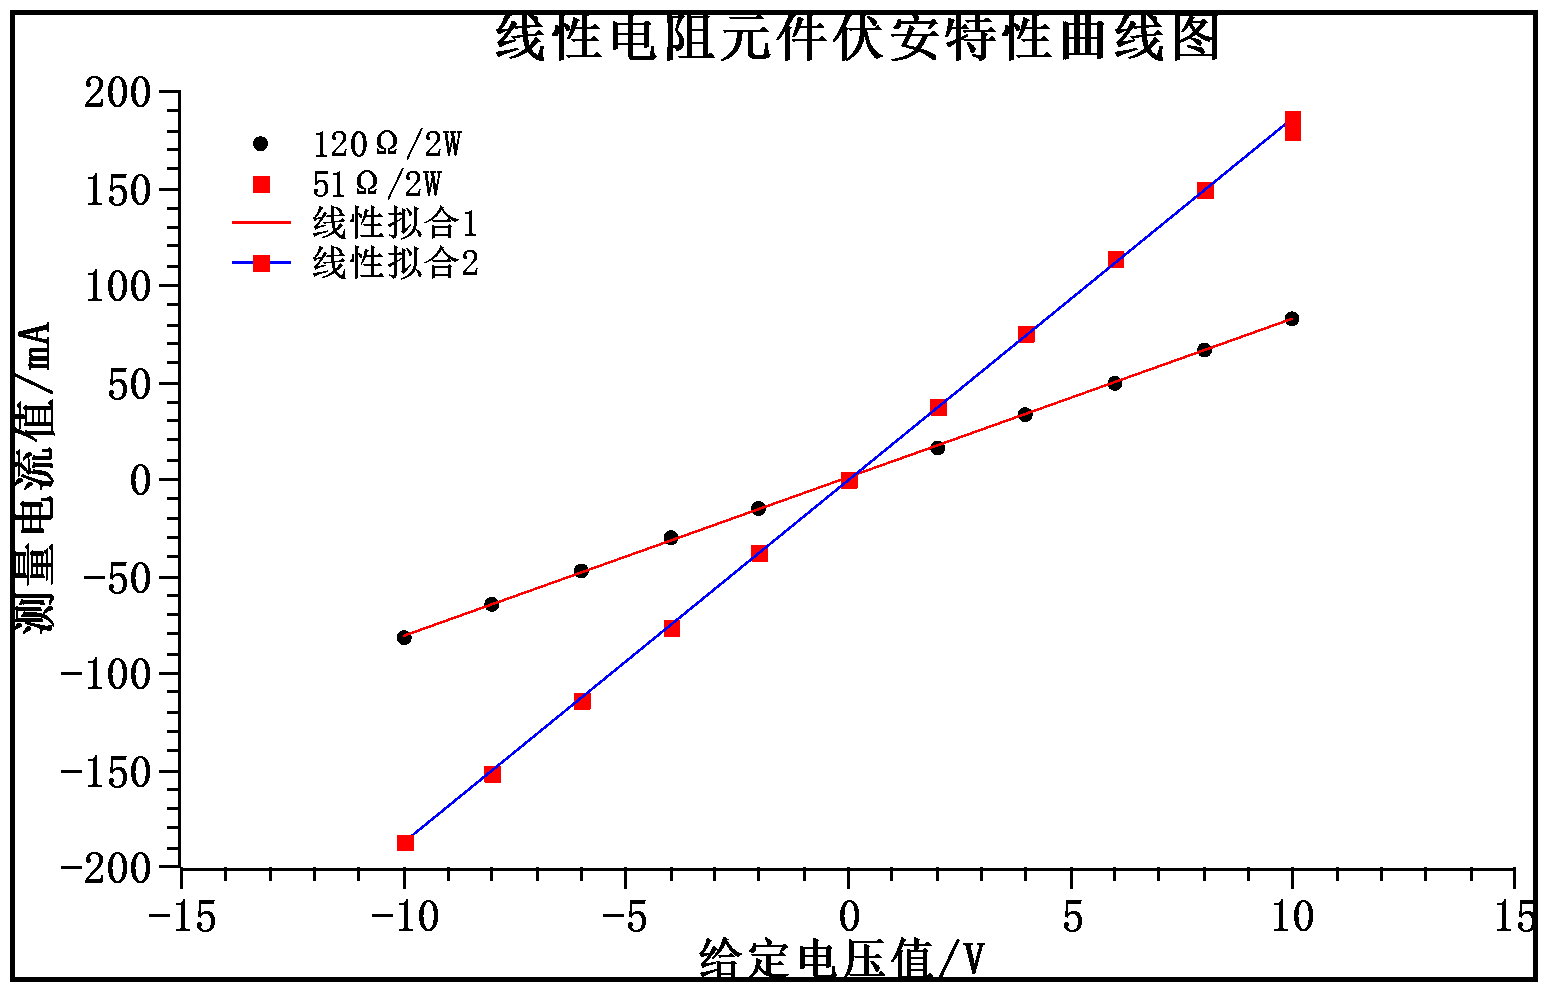
\includegraphics[width=\textwidth-40mm]{002}\\
        \bfseries\zihao{5}\songti 图2:线性电阻元件伏安特性曲线结果图(电流表外接法)
    \end{center}
    \newpage
    \item 根据实验表格3,4(电压表外接法),对上进行同样处理,误差来源分析同上,此处不再赘述。结果图如下图3所示。\\ 拟合结果:$120\Omega/2W$:I=7.699U+0.285,$R^2=0.9996$ \\ $50\Omega/2W$:I=16.810U-5.885,$R^2=0.9997$
    \begin{center}
        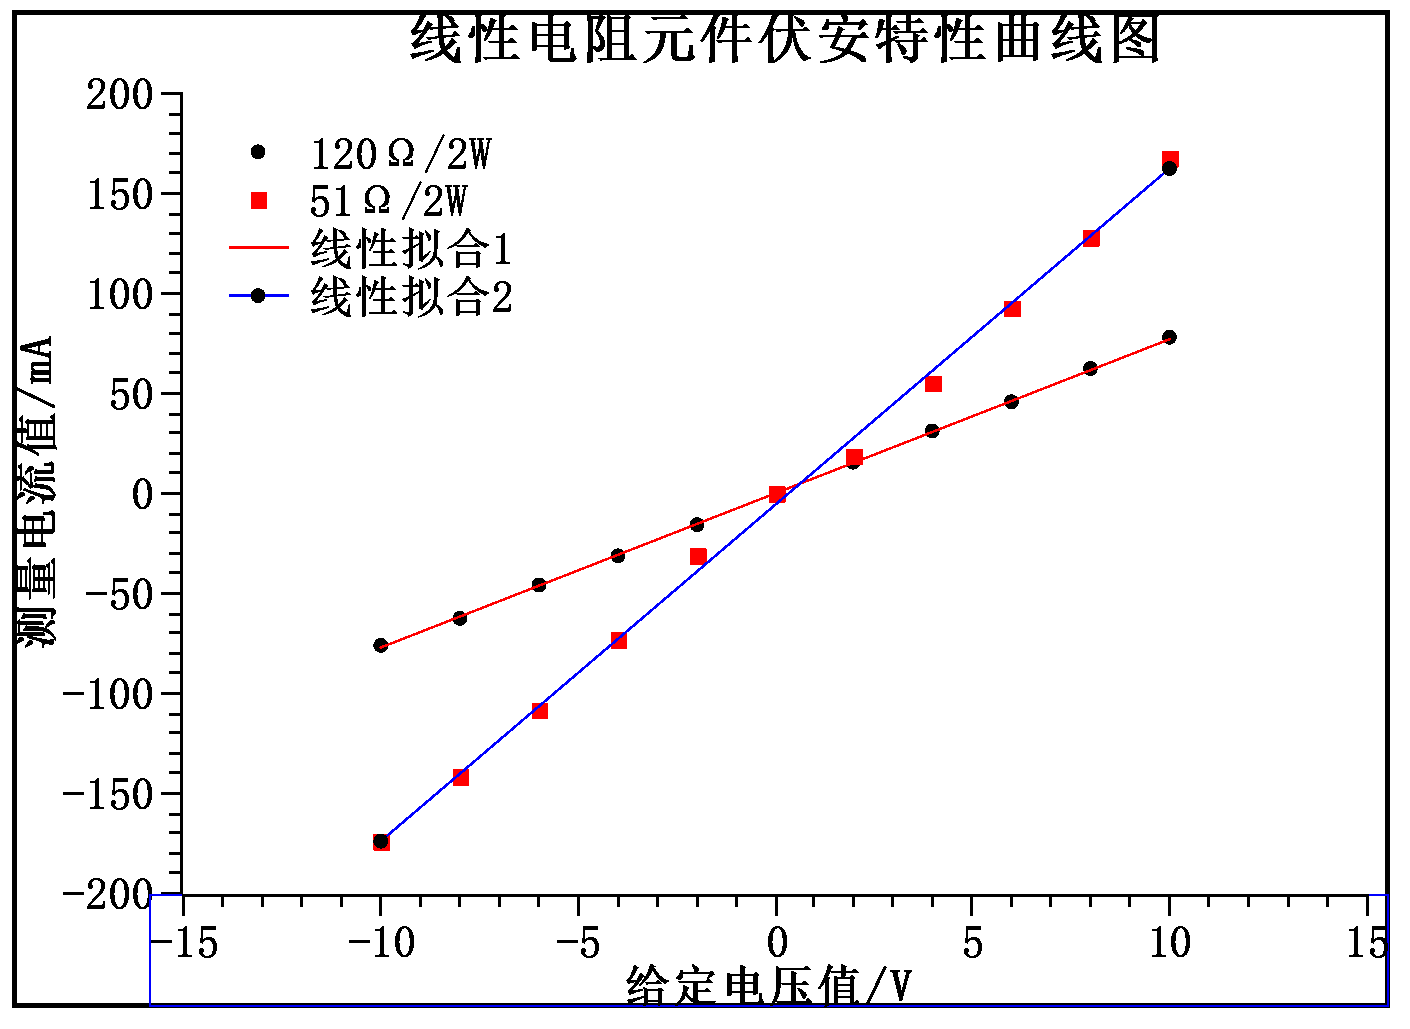
\includegraphics[width=\textwidth-40mm]{003}\\
        \bfseries\zihao{5}\songti 图3:线性电阻元件伏安特性曲线结果图(电压表外接法)
    \end{center}
    \item 对上述两种方法进行比较,其拟合结果的斜率与阻值有一定相关性,根据欧姆定律,可将其视为反比关系。对于同一元件,电流表外接法的测得的斜率大于电压表外接法测得的斜率,则电流表外接法的测得的电阻相较于电压表外接法偏小。
    \item 从原理上分析,电流表外接法中,电压表测得的是待测元件两侧的实际电压,但是电流表测得的电流相较于实际电流偏大,故计算得到的电阻相较于真实值偏小。同理分析电压表外接法,此时电压值偏大,电流值为真实值,则测得的电阻结果相较于真实值偏大。综上,三个值的关系为:电流表外接法结果$<$真实值$<$电压表外接法结果。\\此处分析与测量结果相印证。
\end{enumerate}
\newpage
\begin{flushleft}
    \bfseries\zihao{-4}\songti 【实验二结果分析】
\end{flushleft}
\begin{enumerate}
    \item 对D3二极管IN5401电压表外接法与电流表外接法的结果作图,结果如下四图所示(正向,反向分别作图),反向的伏安特性曲线相较于正向的变化可视为其几乎与X轴重合,故此处分开作图。
    \begin{center}
        \fbox{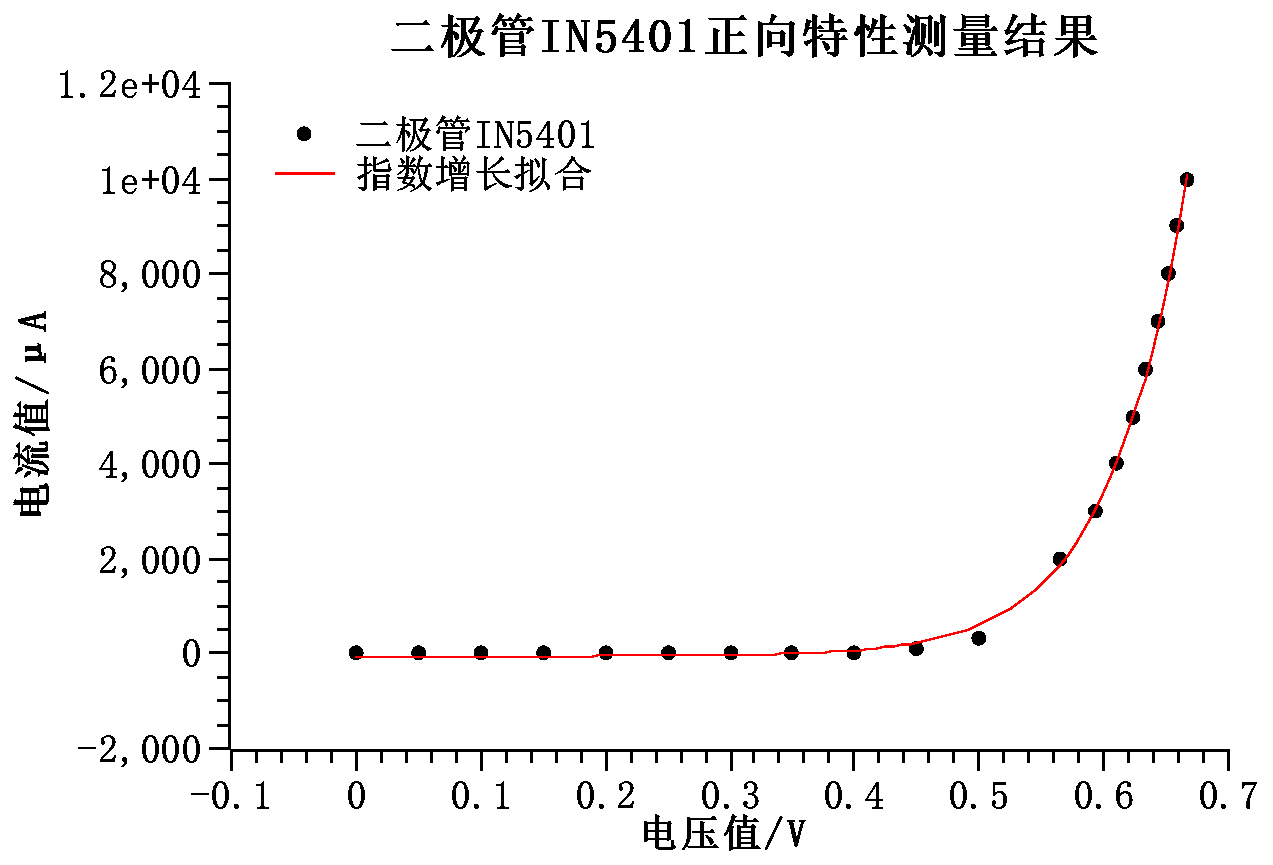
\includegraphics[width=\textwidth-40mm]{004}}\\ 
        \bfseries\zihao{5}\songti 图4:二极管IN5401正向伏安特性曲线结果图(电压表外接法)
    \end{center}
    \begin{center}
        \fbox{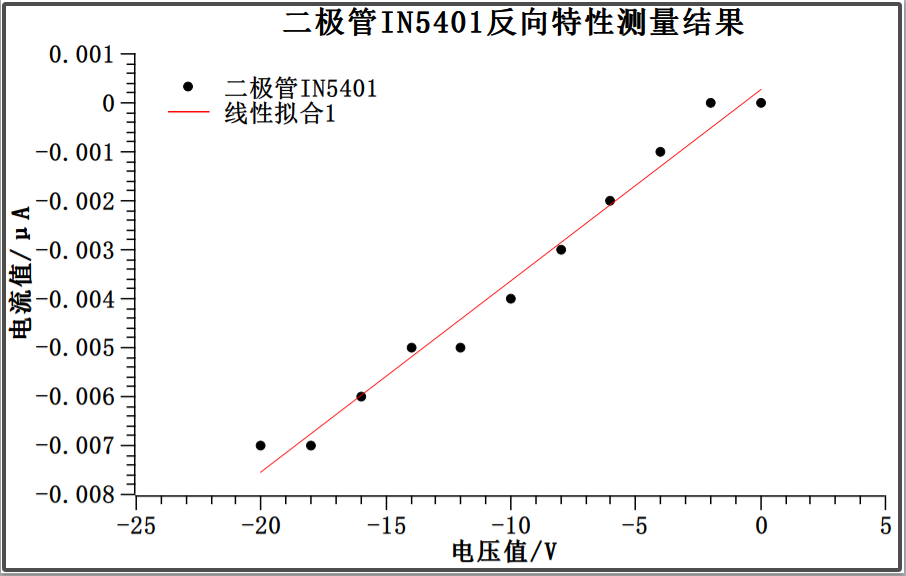
\includegraphics[width=\textwidth-40mm]{005}}\\
        \bfseries\zihao{5}\songti 图5:二极管IN5401反向伏安特性曲线结果图(电压表外接法)
    \end{center}
    \begin{center}
        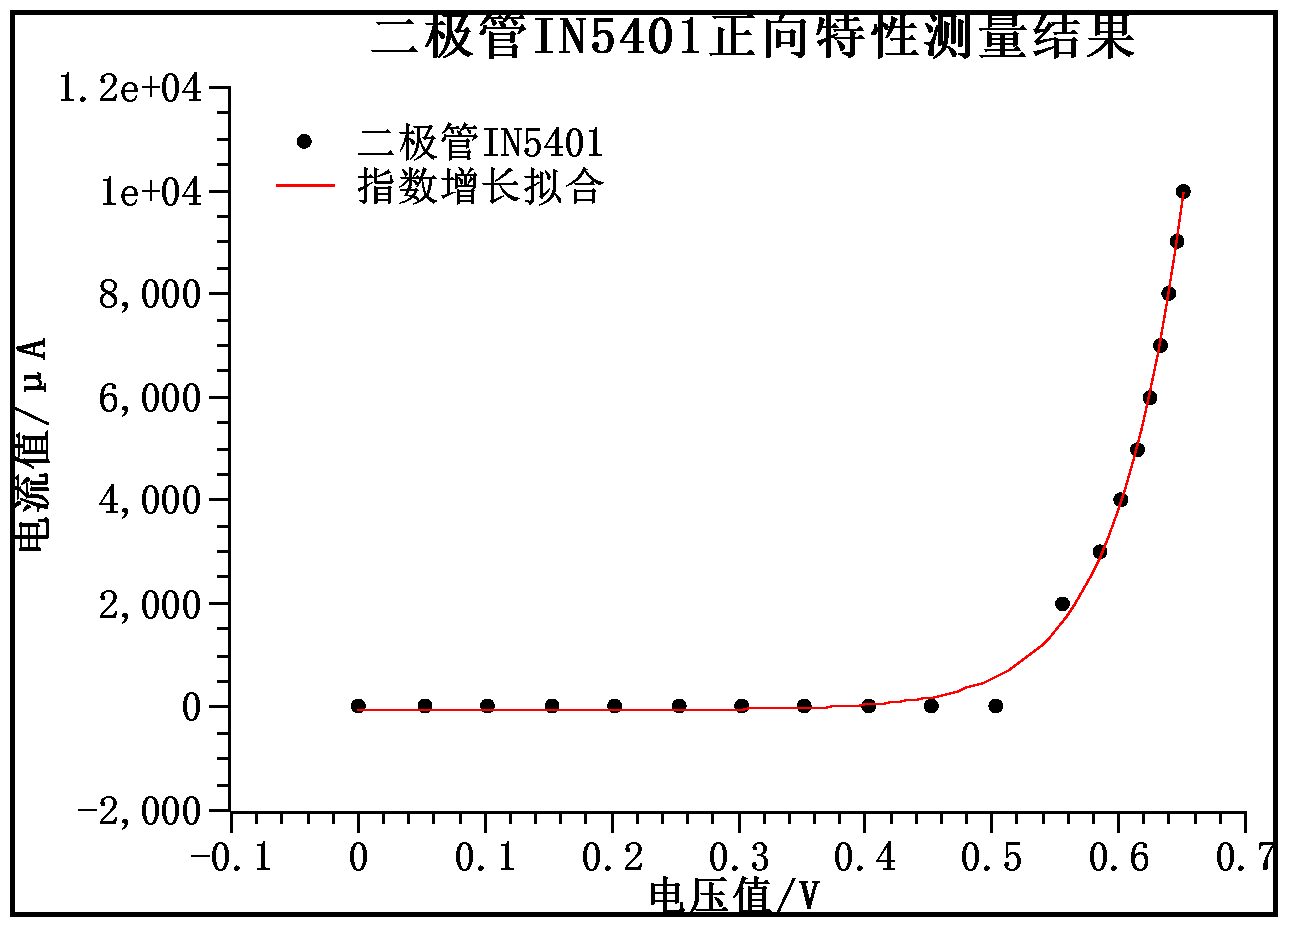
\includegraphics[width=\textwidth-40mm]{006}\\
        \bfseries\zihao{5}\songti 图6:二极管IN5401正向伏安特性曲线结果图(电流表外接法)
    \end{center}
    \begin{center}
        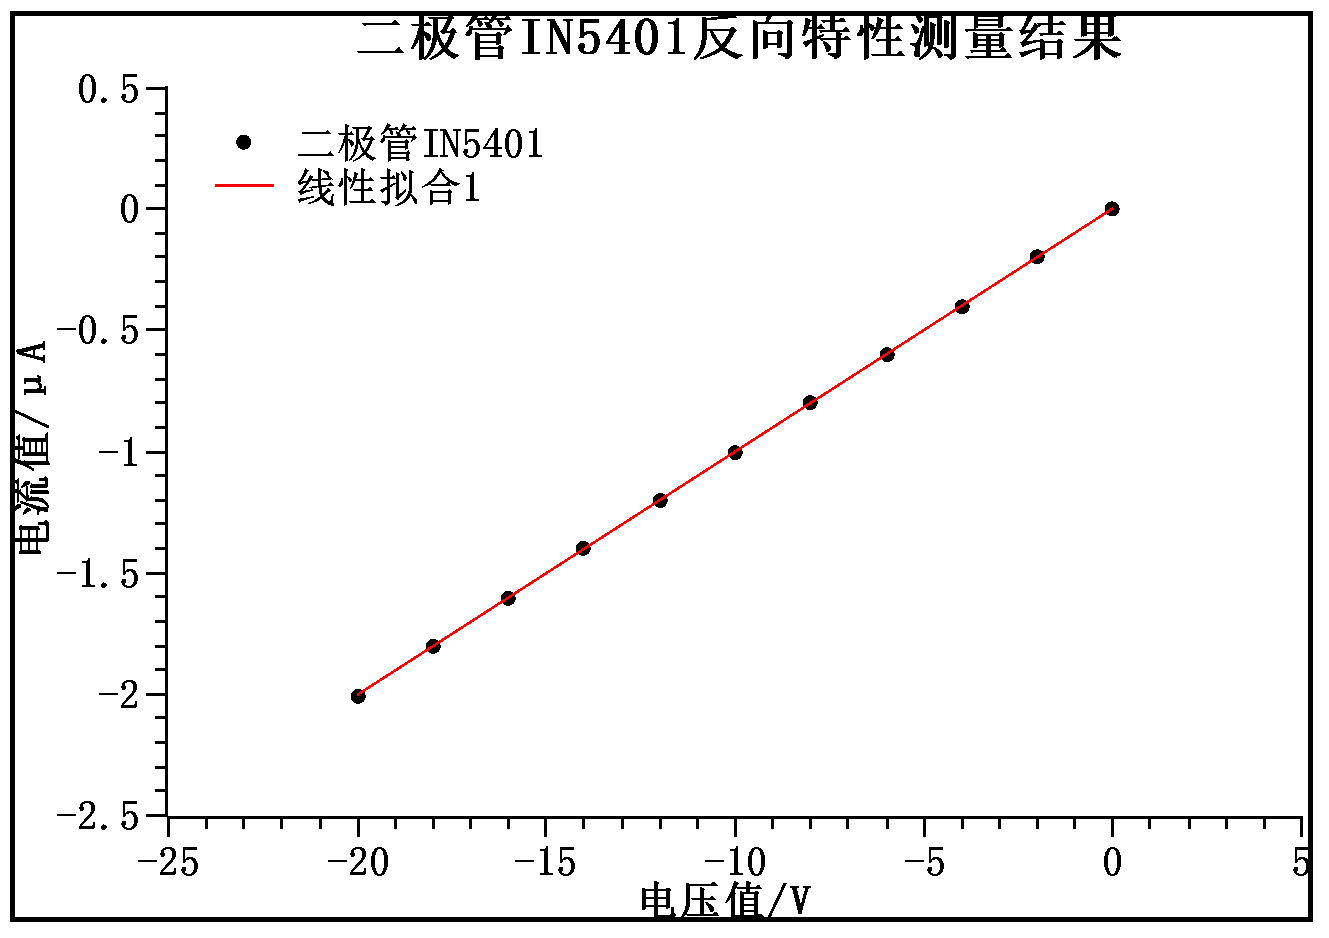
\includegraphics[width=\textwidth-40mm]{007}\\
        \bfseries\zihao{5}\songti 图7:二极管IN5401反向伏安特性曲线结果图(电流表外接法)
    \end{center}
    \item 观察到二极管IN5401在反向电压时几乎没有电流通过,正向电压时一开始的电流值较小,到约0.5V至0.6V的区间时其电阻值发生突变,伏安曲线的斜率忽然增大。
    \item 注意到电流表外接法的结果在反向的时候表现出的线性比电压表外接法强,这与仪器的分辨率有关。在电压表外接法的情况下,电流表直接测量通过元件电流,其电流大小几乎可忽略不计,而电流表外接法,其测量的对象包括了电压表的分流,其相较于元件的反向电流更大,则此时满足线性关系的可能更应该是电压表而非元件。这也进一步印证了前文的结论。
    \newpage
    \item 对D4发光二极管作图同上,得到如下四个结果图。
    \begin{center}
        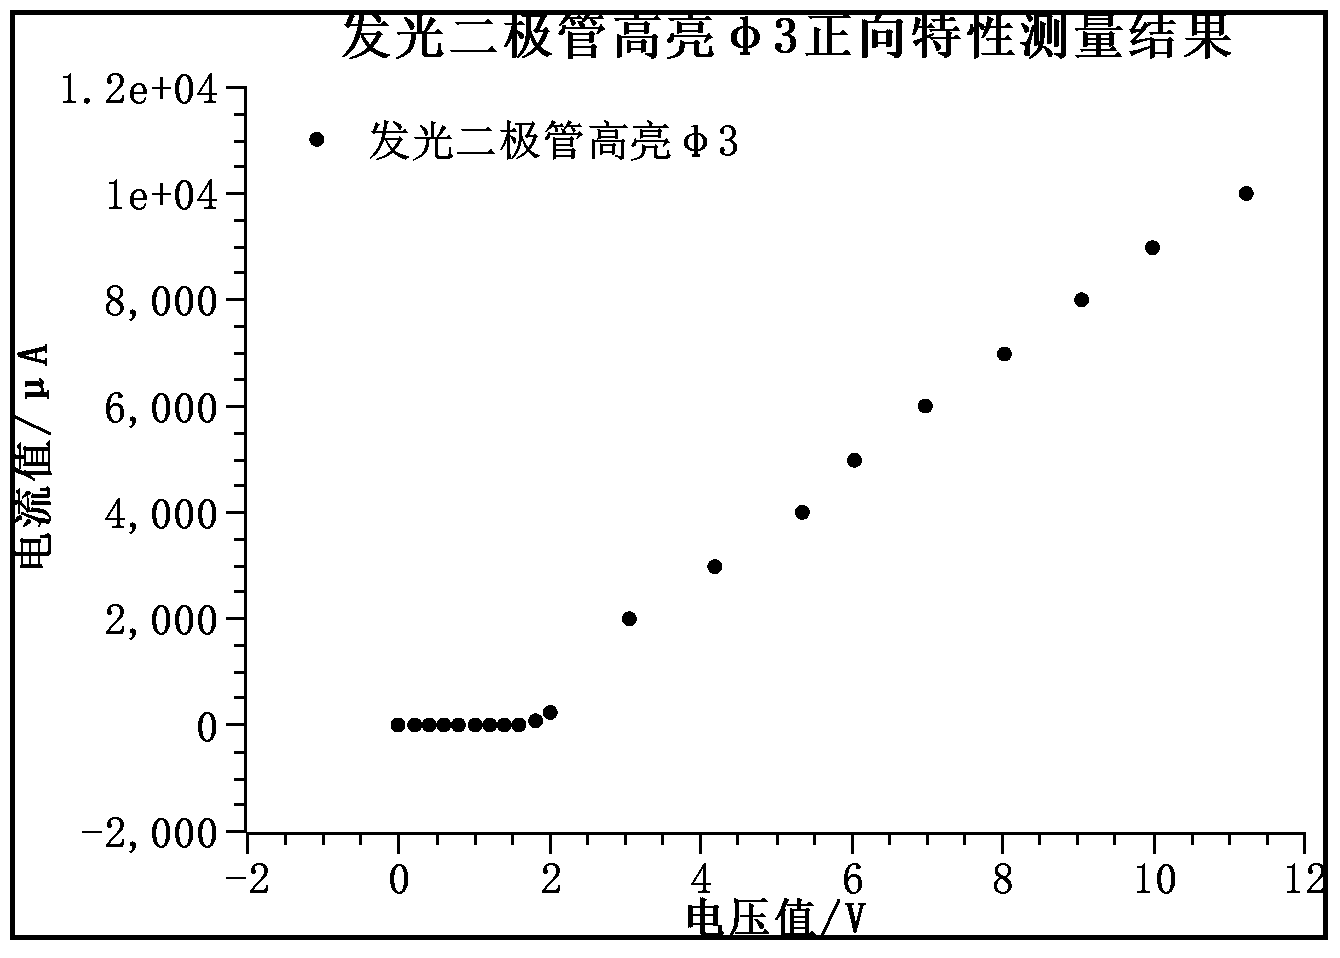
\includegraphics[width=\textwidth-40mm]{008}\\ 
        \bfseries\zihao{5}\songti 图8:发光二极管高亮$\phi$3正向伏安特性曲线结果图(电压表外接法)
    \end{center}
    \begin{center}
        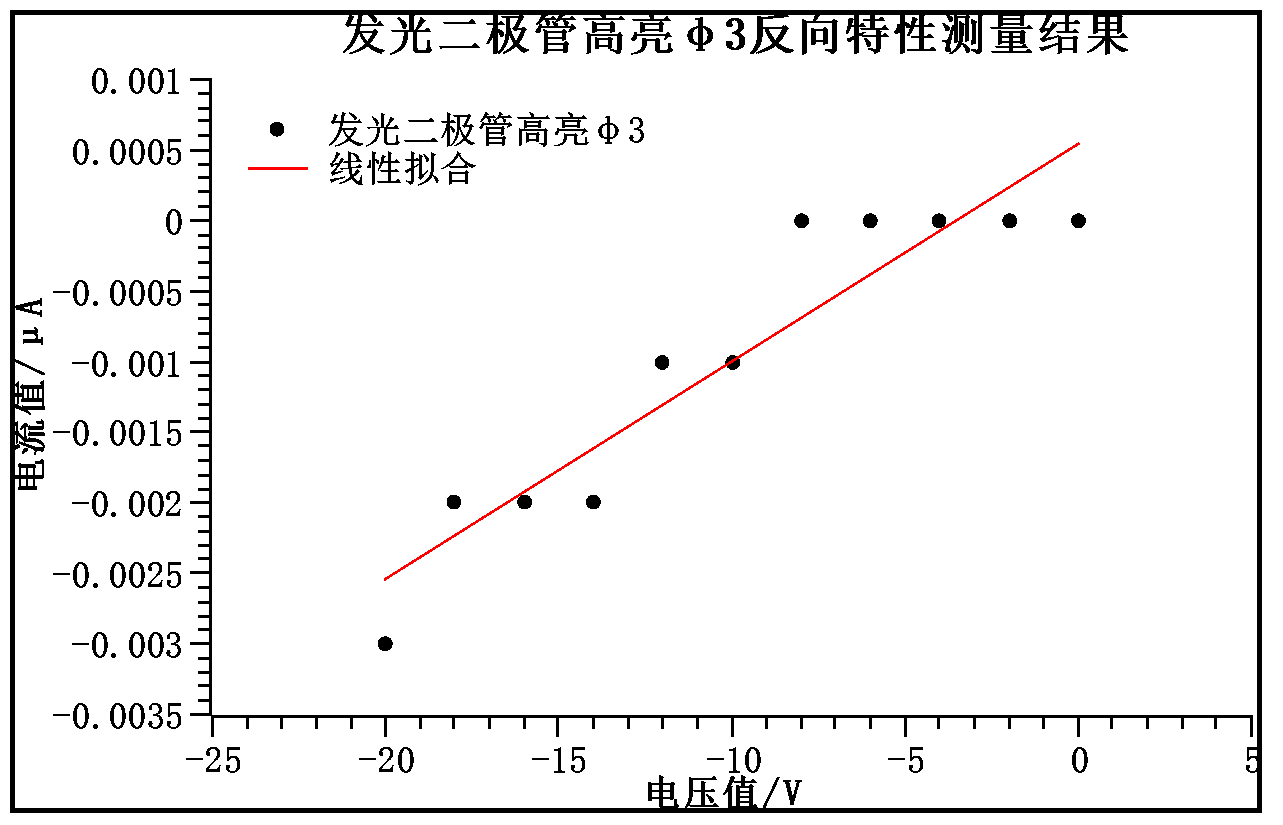
\includegraphics[width=\textwidth-40mm]{009}\\ 
        \bfseries\zihao{5}\songti 图9:发光二极管高亮$\phi$3反向伏安特性曲线结果图(电压表外接法)
    \end{center}
    \begin{center}
        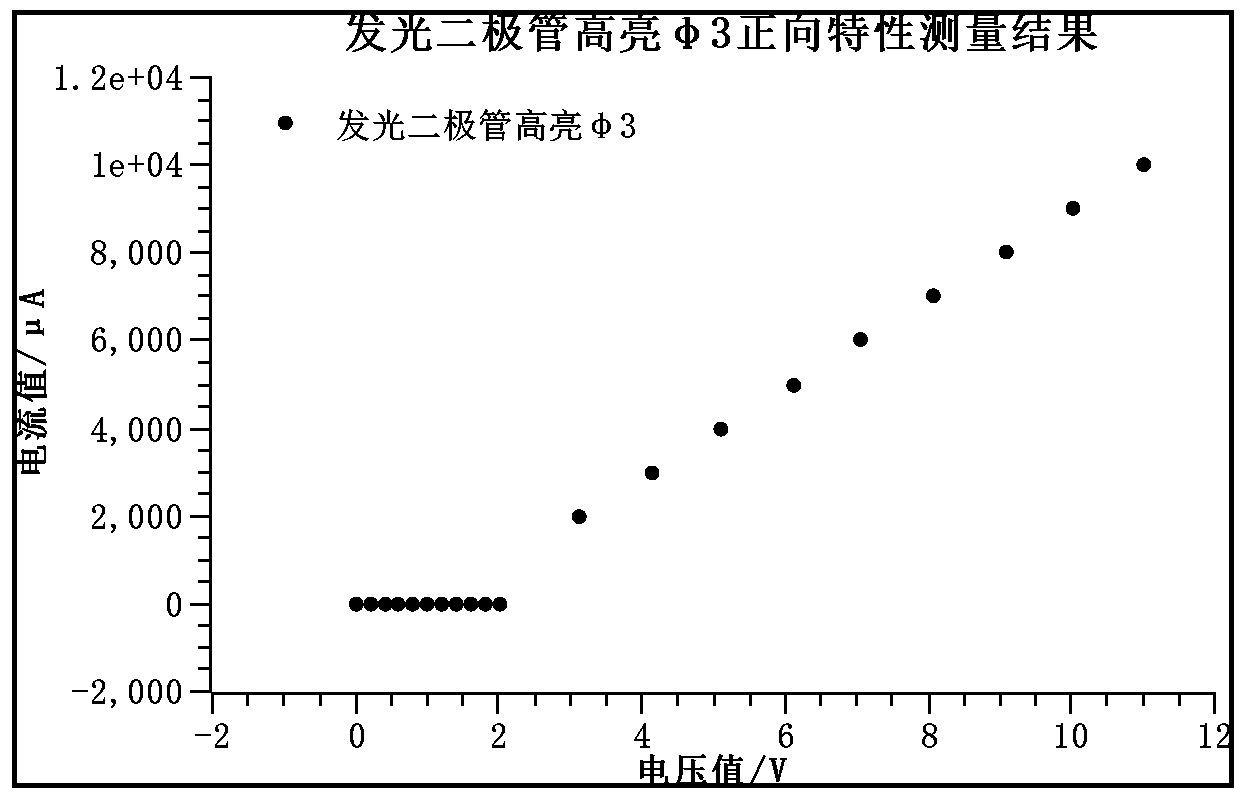
\includegraphics[width=\textwidth-40mm]{010}\\ 
        \bfseries\zihao{5}\songti 图10:发光二极管高亮$\phi$3正向伏安特性曲线结果图(电流表外接法)
    \end{center}
    \begin{center}
        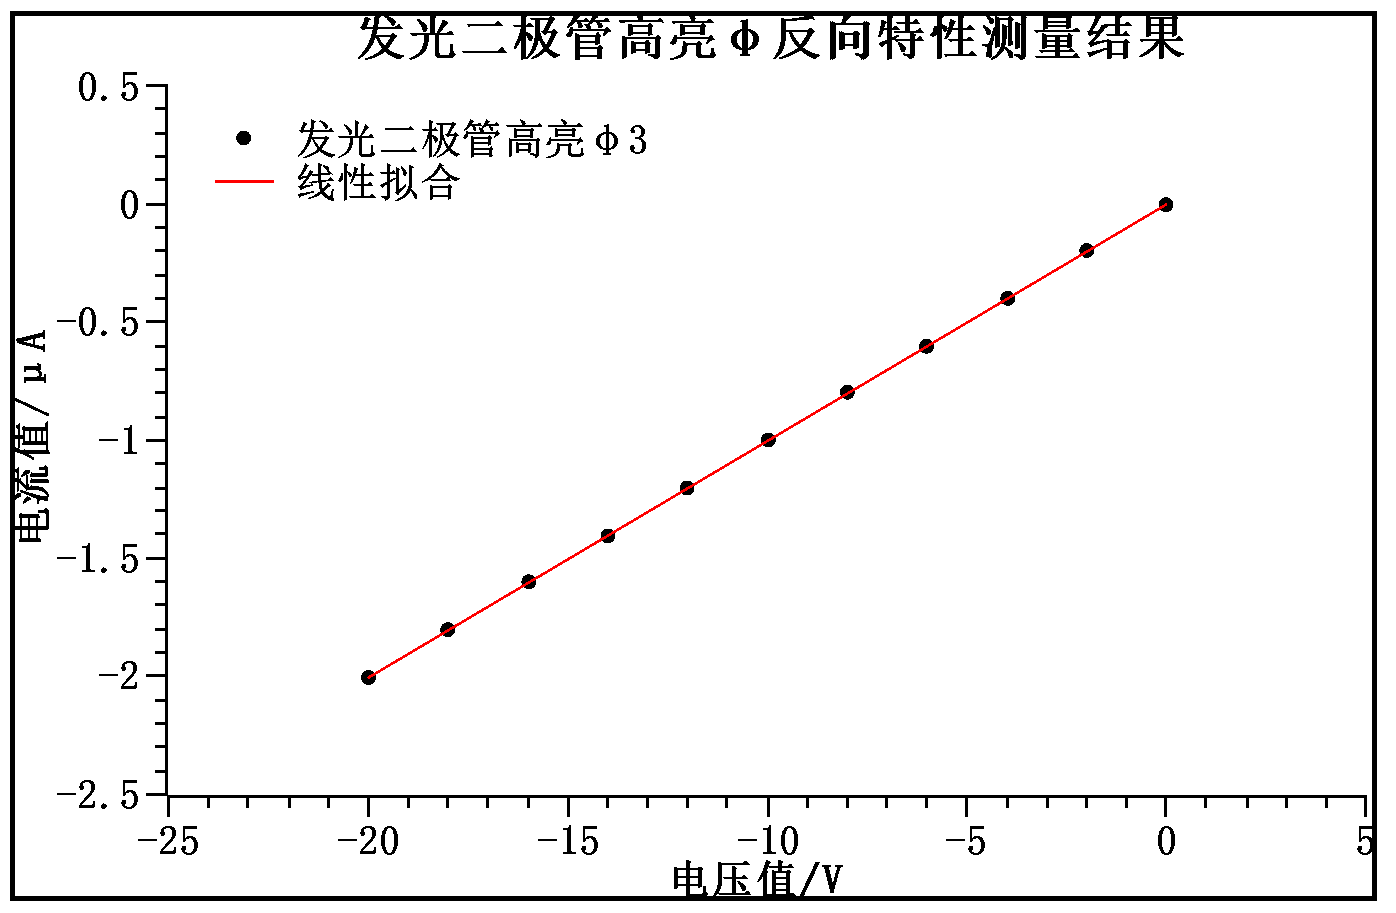
\includegraphics[width=\textwidth-40mm]{011}\\ 
        \bfseries\zihao{5}\songti 图11:发光二极管高亮$\phi$3反向伏安特性曲线结果图(电流表外接法)
    \end{center}
    \item 注意到发光二极管高亮$\phi$3的正向伏安特性,在约2.0V以下的部分其斜率变化较小,在2V左右出现拐点,斜率发生突变,后续呈线性关系。若想更加精细得到拐点的具体情况应当继续增补中间空缺部分的数据点。
    \item 通过反向的伏安特性结果可以得到与D3相同的结论,此处不再赘述。两处的电流表外接法伏安特性曲线线性相关性太低,拟合无实际意义。
    \item 误差来源分析同上,此处不再赘述。
\end{enumerate}

\newpage
\section{思考题}
\begin{enumerate}
    \item 电阻元件、二极管伏安特性的区别和测试方法。\par 电阻元件的电阻阻值维持在一个稳定的值而不会随着两端电压,通过电流的变化而改变,反映到伏安特性曲线上其表现为线性直线。二极管的伏安特性表现,在反向电压的情况下其内部几乎没有电流通过,在正向电压的条件下,其电阻阻值先大后小,表现在伏安特性曲线上,表现为某一电压值附近斜率发生突变,不再满足原本的线性关系。
    \item “开路”:指的是电阻趋近于无穷大,支路中不再有电流通过的情况;“短路”指的是电阻趋近于零的情况,相当于导线。
    \item 可调三端电阻可以起到消振、限流、电压调节、电流调节等,消振作用指可调三端电阻用于防止电路中出现的高频振荡,稳定电路;限流作用指可调三端电阻用于限制电流大小,防止电流过大导致的电路损坏。其余则是其通过改变自身电阻阻值来调整电路中的变量。
    \item 电流表应与被测元件串联,电压表应与被测元件并联,电流表、电压表都有内阻,电流表内阻应越小越好,电压表内阻应越大越好。\\电流表内阻小,则其分压小,电压表示数越接近于待测元件两端电压真实值。电压表内阻大,则其分流越小,电流表测量时越接近于通过待测元件的电流真实值。
    \item 电流表内阻大,电压表内阻小,会导致测量得到的结果与真实值有明显偏差,电压表外接法受电流表内阻大影响,其测得的电压值相较真实值偏大,进而导致测得电阻偏大。电流表外接法则受电压表内阻小影响,测得电流相较于真实值偏大,进而导致测得电阻偏小。
    \item 元件阻值小时,其应当采用电流表外接法,此时其所在支路的电流值大,电压分流作用小,更接近真实值。元件阻值大时,应当采用电压表外接法,此时其所分压电压值大,电流表分压作用小,更接近真实值。
\end{enumerate}

\section{实验心得}
本次实验中对于非线性电路元件的伏安特性曲线的测量仍有不足,虽然对测量方案进行了补充,测量了中间拐点处附近的电压电流值,但是所得到的结果并不理想,可能有仪器测量本身带来的误差等因素导致的影响。可以进一步优化实验过程,高效率地完成实验,并将可能带来误差的因素降到最低以得到更加合理的结果。

\newpage
\begin{center}
    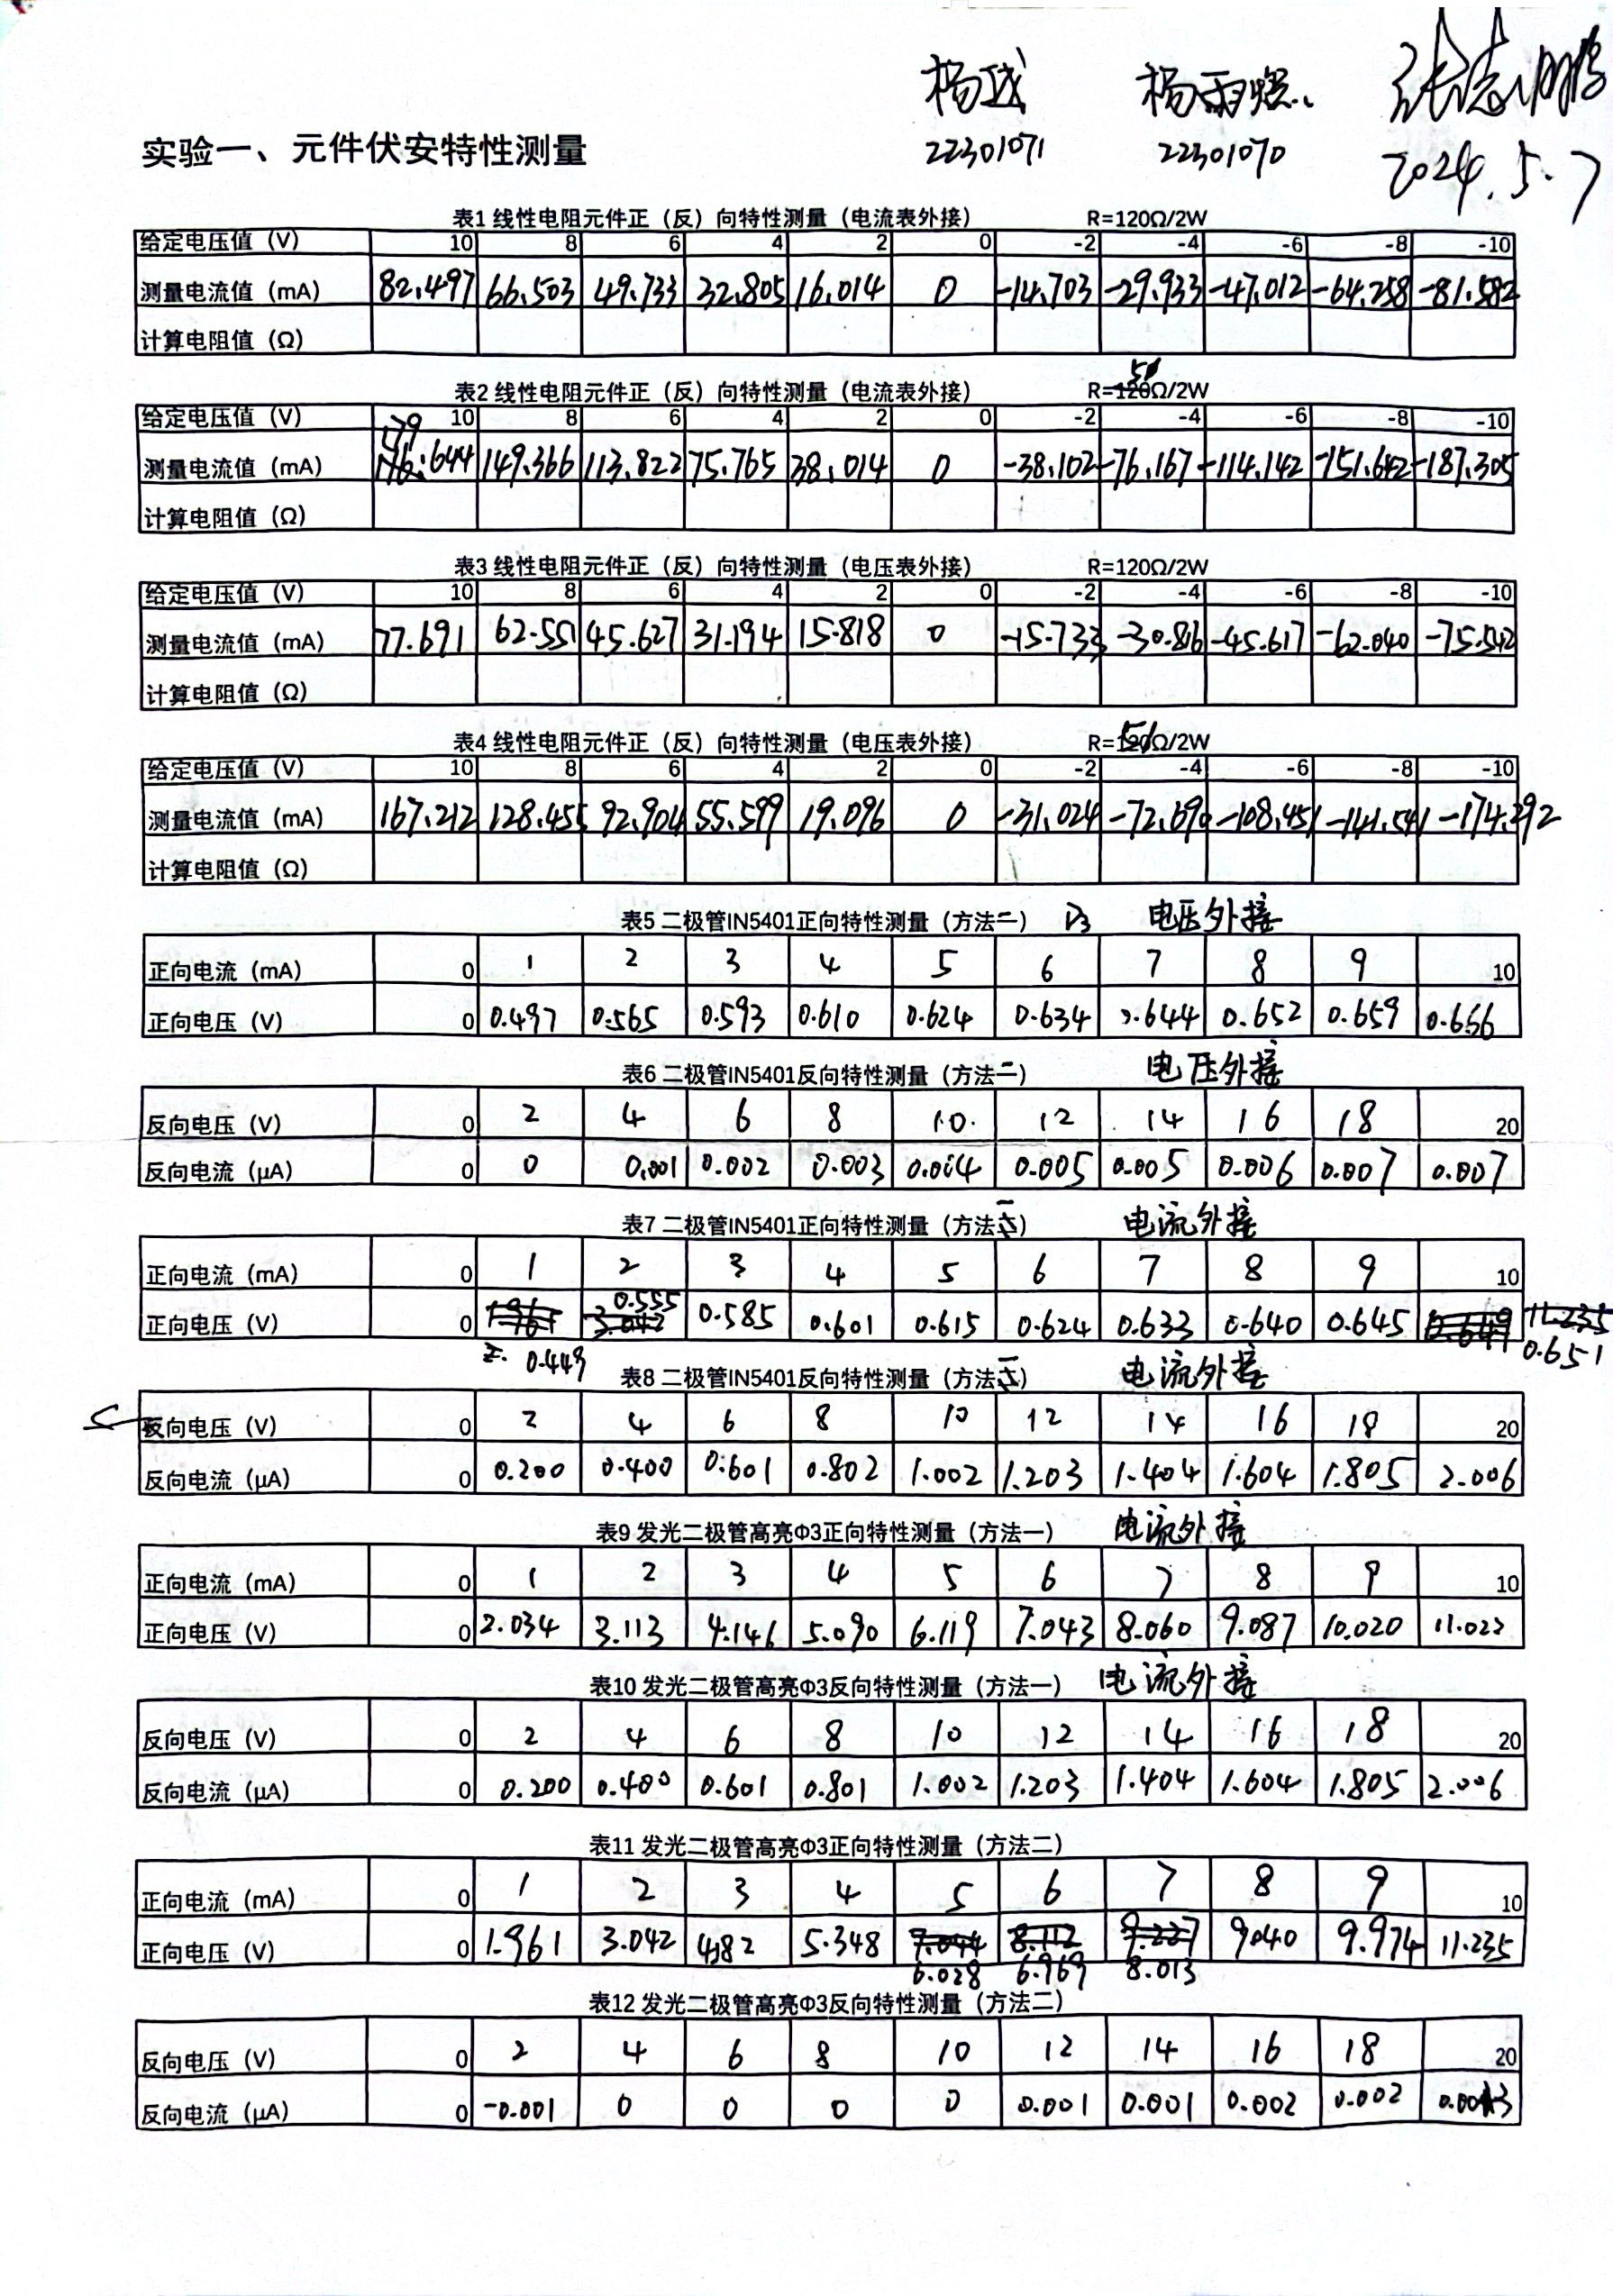
\includegraphics[width=\textwidth]{012}\\
    \newpage
    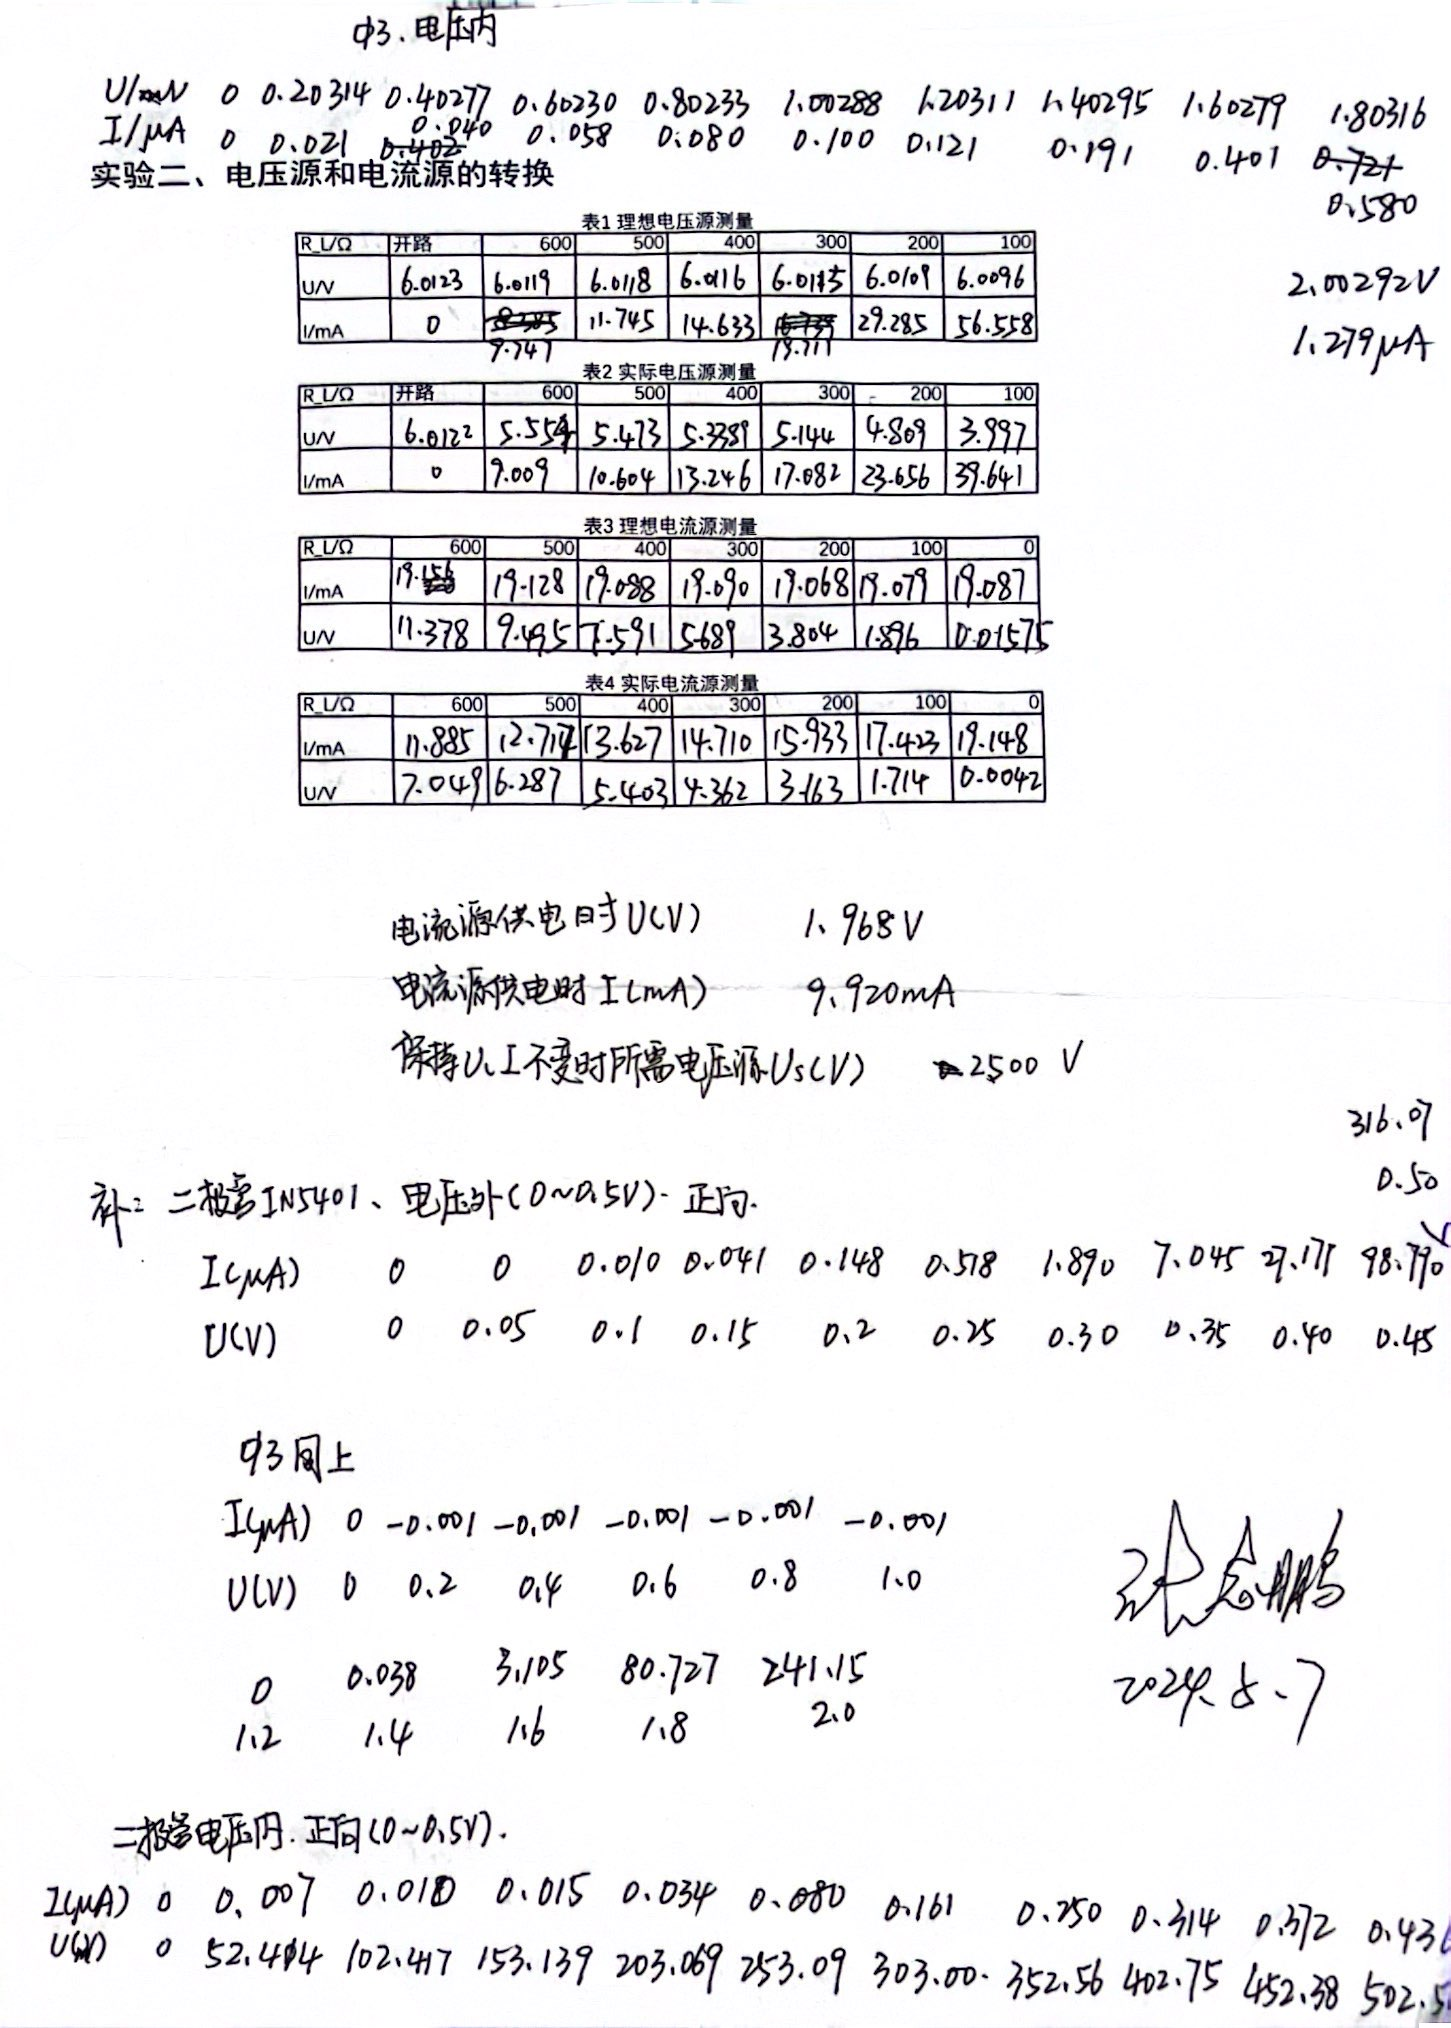
\includegraphics[width=\textwidth]{013}\\
\end{center}

\end{document}